\documentclass[12pt]{article}
\usepackage{amssymb,mathtools}
\usepackage[margin=1in]{geometry}
\usepackage{fancyhdr}
\usepackage{circuitikz}
\usepackage{graphicx}
\graphicspath{ {/Users/GA/Deep_Neural_Nets/HW5/code/Figures/} }
\usepackage{amsmath}
\usepackage{ragged2e}
\usepackage{subcaption} 
\usepackage{float}
\usepackage{bm}
\usepackage{cancel}
\pagestyle{fancy}
\usepackage[shortlabels]{enumitem}
\usepackage{mathtools}
\newcommand*{\permcomb}[4][0mu]{{{}^{#3}\mkern#1#2_{#4}}}
\newcommand*{\Comb}[2]{{}^{#1}C_{#2}}%
\DeclarePairedDelimiter\ceil{\lceil}{\rceil}
\DeclarePairedDelimiter\floor{\lfloor}{\rfloor}
\setlength{\headheight}{15 pt}
\lhead{Andrej Ili\'c, Georgy Antonov}
\chead{HW 5}
\rhead{Deep Neural Networks}

\begin{document}\noindent


\noindent\textbf{Question 1. Logistic Regression - Theory.}
\begin{enumerate}[a)]
    \item 
    Due to binarity of $y$ we can rewrite the definition as 
$$P(y = y^{(i)}  \mid \bm{x}^{(i)}, \bm{\theta}) =  y^{(i)}  \sigma (\bm{\theta}^T \bm{x}^{(i)}) + 
(1-y^{(i)}) (1- \sigma (\bm{\theta}^T \bm{x}^{(i)}))
$$
One of the summands will always cancel, reducing the expression to the given definition of the distribution.
 \item Let's first tackle the derivative 
 $\frac{\partial \log (\sigma(\bm{\theta}^T \bm{x}^{(i)})))}{\partial \theta_j  }$.
 $$
 \frac{\partial \log (\sigma(\bm{\theta}^T \bm{x}^{(i)})))}{\partial \theta_j  }
 = \frac{\partial \log (\sigma(\bm{\theta}^T \bm{x}^{(i)}))}{\partial(\sigma(\bm{\theta}^T \bm{x}^{(i)}))}
 \frac{\partial( \sigma(\bm{\theta}^T \bm{x}^{(i)}))}{\partial( \bm{\theta}^T \bm{x}^{(i)})}
 \frac{\partial( \bm{\theta}^T \bm{x}^{(i)})}{\partial( \theta_j )}$$
 Using the derivative of the sigmoid identity (page 31, lecture 3) we proceed 
 $$=
 \frac{1}{\sigma(\bm{\theta}^T \bm{x}^{(i)})}\sigma(\bm{\theta}^T \bm{x}^{(i)}) (1-\sigma(\bm{\theta}^T \bm{x}^{(i)})) {x}^{(i)}_j
 = (1-\sigma(\bm{\theta}^T \bm{x}^{(i)})) {x}^{(i)}_j $$
 Similarly we have
 $$\frac{\partial \log (1 - \sigma(\bm{\theta}^T \bm{x}^{(i)})))}{\partial \theta_j  } = 
 \frac{1}{1-\sigma(\bm{\theta}^T \bm{x}^{(i)})}
\sigma(\bm{\theta}^T \bm{x}^{(i)}) (\sigma(\bm{\theta}^T \bm{x}^{(i)})-1) {x}^{(i)}_j $$ $$
= - \sigma(\bm{\theta}^T \bm{x}^{(i)}) {x}^{(i)}_j 
 $$
 Then 
 $$\frac{\partial  (\log {P(\bm{y}  \mid \bm{X}, \bm{\theta})})}{\partial \theta_j}
 = \sum_i y^{(i)} \frac{\partial \log (\sigma(\bm{\theta}^T \bm{x}^{(i)})) }{\partial\theta_j }
 +
 (1-y^{(i)}) \frac{\partial \log (1- \sigma(\bm{\theta}^T \bm{x}^{(i)})) }{\partial \theta_j }$$
 $$=
 \sum_i y^{(i)} (1-\sigma(\bm{\theta}^T \bm{x}^{(i)})) {x}^{(i)}_j 
 - 
 (1-y^{(i)}) \sigma(\bm{\theta}^T \bm{x}^{(i)}) {x}^{(i)}_j 
 $$
 $$ = \sum_i {x}^{(i)}_j  (y^{(i)}  - \sigma (\bm{\theta}^T \bm{x}^{(i)}))$$
  \item 
  For total degree of $i$ there exists
  $i+1$ combinations of $x_1$ and $x_2$ powers (via elementary combinatorics). Therefore the total size of the new 
  $\hat{\bm{\theta}}$ is going to be 
  $$\sum_{i=0}^{d} i+1 = 1 + \frac{ d (1 + d)}{2} $$
  We also expand $\hat{\bm{x}}$ to accommodate the combinations of the higher powers of 
  features and it is going to have the same size as $\hat{\bm{\theta}}$. To order the elements of the 
  two vectors we can map $x_1^ix_2^j$ to $\hat{x}_{i\cdot d + j}$
  with the corresponding weight $\hat{\bm{\theta}}_{i\cdot d + j}$.
   
\end{enumerate}
\noindent\textbf{Question 2. Logistic Regression Implementation. }
\begin{enumerate}
    \item[a)] See Figure 1.
    \begin{figure}[h]
        \centering
        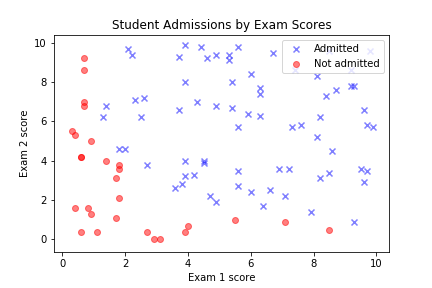
\includegraphics[width=0.8\textwidth]{Train_data.png}
        \caption{Scores on exam 2 plotted against scores on exam 1. Markers indicate admission outcome. Data from the training dataset.}
    \end{figure}
    \item[For] b), c), d) See the attached files
    \item[e)] See Figure 2.
    \begin{figure}[h]
        \centering
        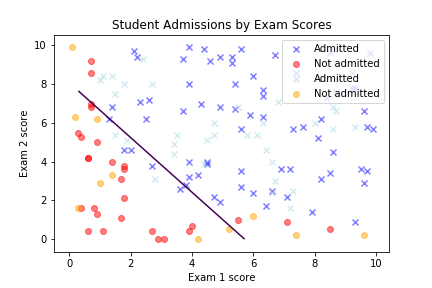
\includegraphics[width=0.8\textwidth]{Decision1_acc0860.png}
        \caption{Linear decision boundary. Data from both training and test datasets. Accuracy obtained was 0.86.}
    \end{figure}
    \item[f)] See Figure. Although asked to plot a decision boundary for either degree 3 or 5 polynomials, the accuracy obtained with a degree 2 polynomial was 1.
    \begin{figure}[h]
        \centering
        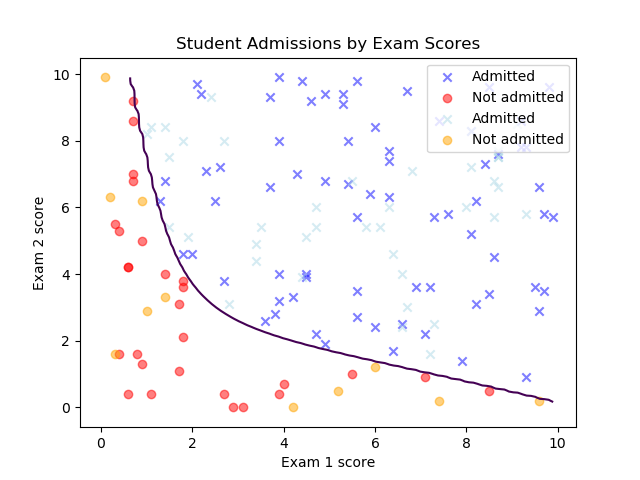
\includegraphics[width=0.8\textwidth]{Decision3_acc1000.png}
        \caption{Decision boundary for a degree 3 polynomial. Accuracy obtained was 1.}
    \end{figure}
\end{enumerate}
\end{document}
